\chapter{Subgraphs}
Rishnak wandered the cemetery, looking for Ajur. As he searched, he saw a headstone with the name Schossow. Rishnak recognized the name from the ``Instant Insanity'' puzzle{\footnote{This is also known as Katzenjammer, (Great) Tantalizer, Face-4, Cube-4, Bognar Balls, Taktikolor, Frantic, Diabolical, Damblocks, and Symington's Puzzle. A patent was awarded to Schossow in 1990.}}, and just as Rishnak was thinking it would be an interesting topic to discuss with Ajur, Jura the dog, eager to explore, nudged Ajur awake from a nap.

Before long, Ajur and Jura were strolling along the path when Rishnak startled Ajur (as ghosts tend to do).

Rishnak asked Ajur what he knew about subgraphs. Ajur said that he was familiar with subsets. ``And since a graph has both a vertex set and an edge set, I think I can deduce what a subgraph is. Given some graph~$G=(V,E)$ with vertex set~$V$ and edge set~$E$, then take any subset~$X$ of~$V$ and consider all edges in~$E$ for which both end vertices are in~$X$.''

Ajur picked up a stick and drew a graph in the dirt [Figure~\ref{3g}].

He said, ``From this first graph, I could define a separate vertex subset~$V'=\{1,2,3,5\}$ to form another graph, say~$G'=(V',E')$, which is a subgraph of the first.''

He drew a second graph [Figure~\ref{3g1}].

\begin{figure}
\begin{center}
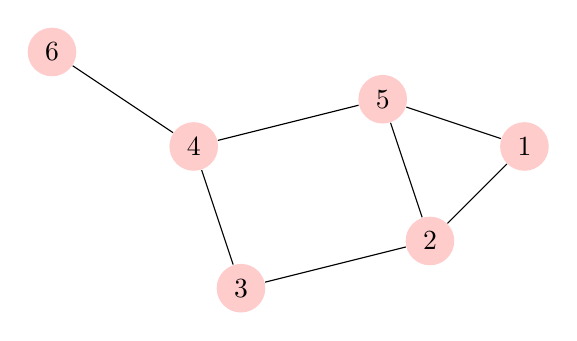
\begin{tikzpicture}
  [scale=.6,auto=left,every node/.style={circle,fill=red!20}]
  \node (n6) at (1,10) {6};
  \node (n4) at (4,8)  {4};
  \node (n5) at (8,9)  {5};
  \node (n1) at (11,8) {1};
  \node (n2) at (9,6)  {2};
  \node (n3) at (5,5)  {3};

  \foreach \from/\to in {n6/n4,n4/n5,n5/n1,n1/n2,n2/n5,n2/n3,n3/n4}
    \draw (\from) -- (\to);

\end{tikzpicture}
\caption{Example graph with six vertices and seven edges}\label{3g}
\end{center}
\end{figure}


\begin{figure}
\begin{center}
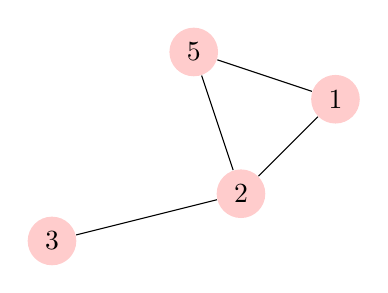
\begin{tikzpicture}
  [scale=.6,auto=left,every node/.style={circle,fill=red!20}]
  %\node (n6) at (1,10) {6};
  %\node (n4) at (4,8)  {4};
  \node (n5) at (8,9)  {5};
  \node (n1) at (11,8) {1};
  \node (n2) at (9,6)  {2};
  \node (n3) at (5,5)  {3};

  \foreach \from/\to in {n5/n1,n1/n2,n2/n5,n2/n3}
    \draw (\from) -- (\to);
\end{tikzpicture}
\caption{Induced subgraph of the graph shown in Figure~\ref{3g}, with vertices in set $V'=\{1,2,3,5\}$ and all edges between these vertices present from the original graph}\label{3g1}
\end{center}
\end{figure}

Rishnak laughed and said that the subgraph Ajur drew was called an \textit{induced subgraph}. He said, ``It is called that because all of the edges are included in the vertex subset. You do have the flexibility of choosing only a subset of these edges, but there is one condition: for each edge in the chosen subset of edges, the end vertices must be in the chosen vertex subset. Let me show you.''

Rishnak drew a graph in the air in a dazzling light display [Figure~\ref{3g2}]. ``Here is a subgraph of your original graph. And note that a subgraph with no vertices and no edges is also an induced subgraph (and subgraph) of any graph.''

\begin{figure}
\begin{center}
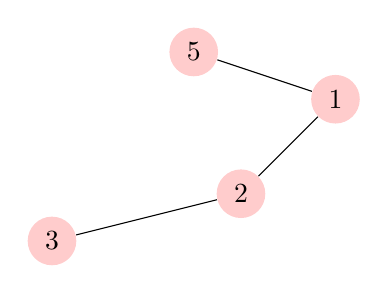
\begin{tikzpicture}
  [scale=.6,auto=left,every node/.style={circle,fill=red!20}]
  %\node (n6) at (1,10) {6};
  %\node (n4) at (4,8)  {4};
  \node (n5) at (8,9)  {5};
  \node (n1) at (11,8) {1};
  \node (n2) at (9,6)  {2};
  \node (n3) at (5,5)  {3};

  \foreach \from/\to in {n5/n1,n1/n2,n2/n3}
    \draw (\from) -- (\to);

\end{tikzpicture}
\caption{A subgraph of Figure~\ref{3g}}\label{3g2}
\end{center}
\end{figure}


%Rishnak said that in a graph having $n$ vertices where the vertices are labeled (have a number/name associated with them), then there are at least $2^n$ subgraphs and exactly $2^n$ induced subgraphs.  There are ${n \choose i}$ ways of choosing $i$ vertices from a given set of $n$ vertices. Once the vertices are chosen, the edges are fixed for an induced subgraph. Since $i$ can vary from 0 to $n$, we get $2^n$ induced subgraphs. Since every induced subgraph is a subgraph (and not every subgraph is not an induced subgraph), we have at least $2^n$ subgraphs.  

Ajur nodded his head and yawned.
Rishnak scowled and said, ``Time to learn something new, Ajur, then see if you can still answer my questions.''

Ajur straightened as Rishnak continued. ``A walk from a vertex~$i$ to a vertex~$j$ is an alternating sequence of vertices and edges. Every edge in that walk is incident between vertices preceding and succeeding that edge. For example, in that graph that you drew''---he pointed down to the dirt [Figure~\ref{3g}]---``a walk from vertex~6 to vertex~1 could be $6-(6,4)-4-(4,3)-3-(3,2)-2-(2,1)-1$. The edges are represented as a vertex pair. And if those edges have names as labels, we could use that label instead. Another walk from vertex~6 to vertex~1 could be $6-(6,4)-4-(4,5)-5-(5,1)-1$.''

Ajur listened intently, then asked, ``Can a walk use the same edge more than once?''

Rishnak said, ``No. The only other condition that a walk has (besides an edge being incident on a preceding and a succeeding vertex) is that all edges must be distinct. The vertices in a walk can be repeated, though. Have a look at this graph.'' In a flash of light, Rishnak drew another graph [Figure~\ref{3g3}]. ``A walk from vertex~1 to vertex~8 could be $1-(1,2)-2-(2,4)-4-(4,6)-6-(6,8)-8-(8,2)-2-(2,3)-3-(3,4)-4-(4,5)-5-(5,6)-6-(6,7)-7-(7,8)-8$.''

Ajur tried to pay attention but was naturally getting bored. He interjected, ``In your walk, you have visited all the edges in the graph, much like the K\"{o}nigsberg Bridge Problem.''\footnote{As mentioned earlier in Chapter 3 [Figure~\ref{kon}].}

\begin{figure}
\begin{center}
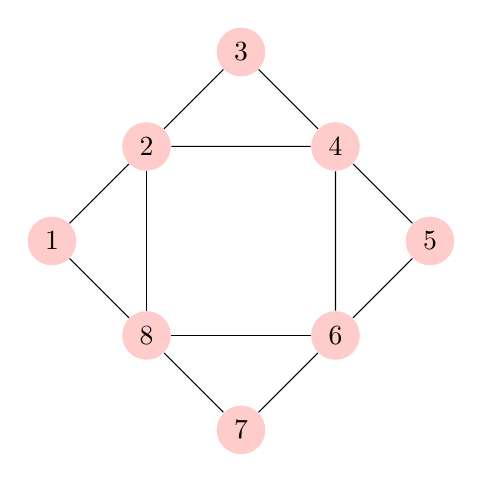
\begin{tikzpicture}
  [scale=.6,auto=left,every node/.style={circle,fill=red!20}]
  \node (n1) at (1,7) {1};
  \node (n2) at (3,9)  {2};
  \node (n3) at (5,11)  {3};
  \node (n4) at (7,9) {4};
  \node (n5) at (9,7)  {5};
  \node (n6) at (7,5)  {6};
  \node (n7) at (5,3)  {7};
  \node (n8) at (3,5)  {8};

  \foreach \from/\to in {n1/n2,n1/n8,n2/n3,n2/n4,n2/n8,n3/n4,n4/n5,n4/n6,n5/n6,n6/n7,n6/n8,n7/n8}
    \draw (\from) -- (\to);

\end{tikzpicture}
\caption{Example graph with eight vertices and 12 edges}\label{3g3}
\end{center}
\end{figure}

Rishnak smiled and nodded. ``And if the starting and ending vertices in a walk are the same, it is known as a closed walk. If all of the edges in a closed walk are distinct, then it is known as a cycle.''

Ajur remembered the idea of a cycle from yesterday's discussion of trees.

Rishnak asked Ajur to list two cycles from the graph that sparkled in front of him [Figure~\ref{3g3}].

Ajur had no trouble at all in listing two cycles as $1-(1,2)-2-(2,8)-8-(8,1)-1$ and $2-(2,4)-4-(4,6)-6-(6,8)-8-(8,2)-2$. Rishnak taught Ajur that often the edges are omitted when describing a walk, so the cycles could be written simply as $(1,2,8,1)$ and $(2,4,6,8,2)$. And even simpler, we can state that a walk is a cycle and omit the repetitive last vertex, so we have cycles $(1,2,8)$ and $(2,4,6,8)$.

Rishnak beamed as he went on.  ``Of course a cycle and a walk are examples of subgraphs with some added conditions. These added conditions make the study of subgraphs very interesting. If in a cycle, all the vertices of the original graph are present, then that cycle is known as a Hamiltonian Cycle. For example, in this graph''---he again referred to the graph that shone in front of him [Figure~\ref{3g3}]---``the cycle $(1,2,3,4,5,6,7,8,1)$ is a Hamiltonian Cycle of this other graph''---he whisked his hands through the air to produce another graph [Figure~\ref{3g4}]---``And if all the edges in a walk are distinct then it is known as a path.''

\begin{figure}
\begin{center}
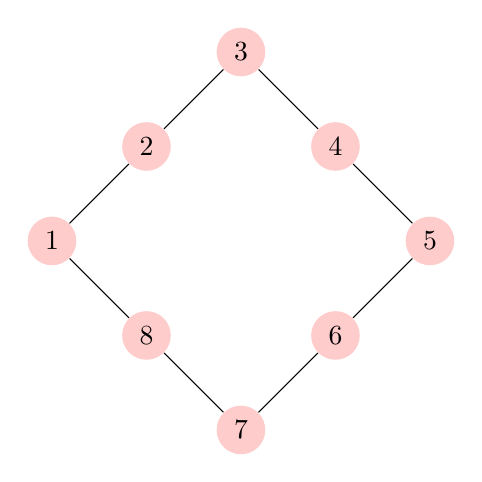
\begin{tikzpicture}
  [scale=.6,auto=left,every node/.style={circle,fill=red!20}]
  \node (n1) at (1,7) {1};
  \node (n2) at (3,9)  {2};
  \node (n3) at (5,11)  {3};
  \node (n4) at (7,9) {4};
  \node (n5) at (9,7)  {5};
  \node (n6) at (7,5)  {6};
  \node (n7) at (5,3)  {7};
  \node (n8) at (3,5)  {8};

  \foreach \from/\to in {n1/n2,n1/n8,n2/n3,n3/n4,n4/n5,n5/n6,n6/n7,n7/n8}
    \draw (\from) -- (\to);

\end{tikzpicture}
\caption{A subgraph of Figure~\ref{3g3}, which forms a Hamiltonian Cycle}\label{3g4}
\end{center}
\end{figure}


Ajur tried to keep up.  ``Okay, so in that first graph''---he pointed to the graph [Figure~\ref{3g3}]---``an example path is $1-(1,2)-2-(2,3)-3$ or simply $(1,2,3)$. Let me draw this path.'' He drew the path in the dirt [Figure~\ref{3g5}].

\begin{figure}
\begin{center}
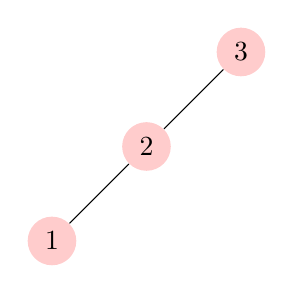
\begin{tikzpicture}
  [scale=.6,auto=left,every node/.style={circle,fill=red!20}]
  \node (n1) at (1,7) {1};
  \node (n2) at (3,9)  {2};
  \node (n3) at (5,11)  {3};

  \foreach \from/\to in {n1/n2,n2/n3}
    \draw (\from) -- (\to);

\end{tikzpicture}
\caption{A subgraph of Figure~\ref{3g3}, which forms a tree}\label{3g5}
\end{center}
\end{figure}

Rishnak nodded, then continued, ``If there is a path between every pair of vertices in a subgraph, then the subgraph is said to be connected. If a subgraph contains no cycles and is connected, the subgraph is a tree. And if such a tree contains all of the vertices then it is known as a spanning tree since it spans all vertices. Watch closely, here's a spanning tree.''

Rishnak transformed the original graph [Figure~\ref{3g3}] into a new one with fewer edges [Figure~\ref{3g6}].

\begin{figure}
\begin{center}
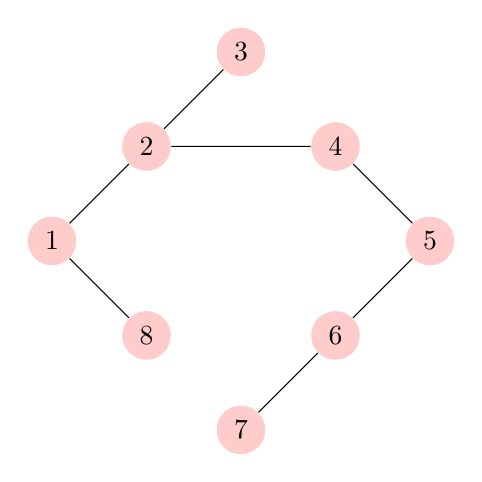
\begin{tikzpicture}
  [scale=.6,auto=left,every node/.style={circle,fill=red!20}]
  \node (n1) at (1,7) {1};
  \node (n2) at (3,9)  {2};
  \node (n3) at (5,11)  {3};
  \node (n4) at (7,9) {4};
  \node (n5) at (9,7)  {5};
  \node (n6) at (7,5)  {6};
  \node (n7) at (5,3)  {7};
  \node (n8) at (3,5)  {8};

  \foreach \from/\to in {n1/n2,n1/n8,n2/n3,n2/n4,n4/n5,n5/n6,n6/n7}
    \draw (\from) -- (\to);

\end{tikzpicture}
\caption{A subgraph of Figure~\ref{3g3}, which forms a spanning tree}\label{3g6}
\end{center}
\end{figure}

Rishnak continued, ``A subgraph in which the degree of every vertex is~1 is said to be a matching. An example of a subgraph that is a matching for this original graph''---he again showed the original graph [Figure~\ref{3g3}]---``is this other graph that contains pairs of vertices.'' Rishnak moved his hands and the graph reduced to one with only three edges [Figure~\ref{3g7}].

``If the subgraph contains all vertices and the degree of every vertex is~1, then it is called a perfect matching. Here's an example of a subgraph that is a perfect matching.'' A new graph appeared, this time with all of the original vertices but only four edges [Figure~\ref{3g8}].

Rishnak asked Ajur how many perfect matchings there were in the original graph [Figure~\ref{3g3}].

Ajur thought for a bit, his brain catching up with everything Rishnak was showing him. He saw that vertices~1, 3, 5, and~7 have degree~2. Therefore, one of those incident on~1, 3, 5, and~7 would have to be selected. ``There are exactly two perfect matchings.''

\begin{figure}
\begin{center}
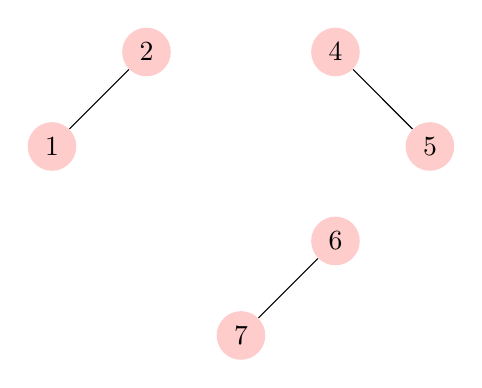
\begin{tikzpicture}
  [scale=.6,auto=left,every node/.style={circle,fill=red!20}]
  \node (n1) at (1,7) {1};
  \node (n2) at (3,9)  {2};
  %\node (n3) at (5,11)  {3};
  \node (n4) at (7,9) {4};
  \node (n5) at (9,7)  {5};
  \node (n6) at (7,5)  {6};
  \node (n7) at (5,3)  {7};
  %\node (n8) at (3,5)  {8};

  \foreach \from/\to in {n1/n2,n4/n5,n6/n7}
    \draw (\from) -- (\to);

\end{tikzpicture}
\caption{A subgraph of Figure~\ref{3g3}, which forms a matching}\label{3g7}
\end{center}
\end{figure}

\begin{figure}
\begin{center}
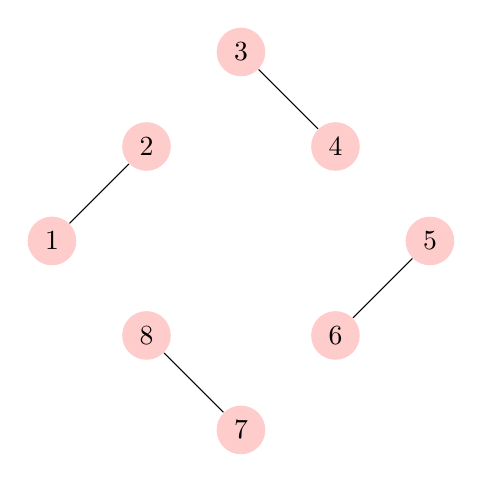
\begin{tikzpicture}
  [scale=.6,auto=left,every node/.style={circle,fill=red!20}]
  \node (n1) at (1,7) {1};
  \node (n2) at (3,9)  {2};
  \node (n3) at (5,11)  {3};
  \node (n4) at (7,9) {4};
  \node (n5) at (9,7)  {5};
  \node (n6) at (7,5)  {6};
  \node (n7) at (5,3)  {7};
  \node (n8) at (3,5)  {8};

  \foreach \from/\to in {n1/n2,n3/n4,n5/n6,n7/n8}
    \draw (\from) -- (\to);

\end{tikzpicture}
\caption{A subgraph of Figure~\ref{3g3}, which forms a perfect matching}\label{3g8}
\end{center}
\end{figure}

Rishnak had more to teach Ajur.  He said, ``A graph is connected if there is a path between every pair of vertices in that graph. Otherwise the graph is disconnected. Watch closely as here are two graphs, the first being a connected graph [Figure~\ref{3g9}], the second a graph that is not connected [Figure~\ref{3g10}].''

\begin{figure}
\begin{center}
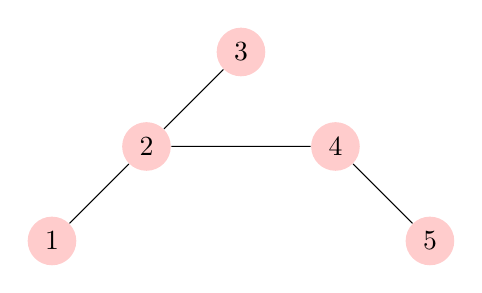
\begin{tikzpicture}
  [scale=.6,auto=left,every node/.style={circle,fill=red!20}]
  \node (n1) at (1,7) {1};
  \node (n2) at (3,9)  {2};
  \node (n3) at (5,11)  {3};
  \node (n4) at (7,9) {4};
  \node (n5) at (9,7)  {5};
\foreach \from/\to in {n1/n2,n2/n3,n2/n4,n4/n5}
    \draw (\from) -- (\to);

\end{tikzpicture}
\caption{A connected graph}\label{3g9}
\end{center}
\end{figure}

\begin{figure}
\begin{center}
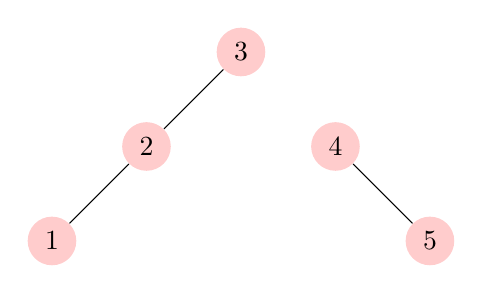
\begin{tikzpicture}
  [scale=.6,auto=left,every node/.style={circle,fill=red!20}]
  \node (n1) at (1,7) {1};
  \node (n2) at (3,9)  {2};
  \node (n3) at (5,11)  {3};
  \node (n4) at (7,9) {4};
  \node (n5) at (9,7)  {5};
\foreach \from/\to in {n1/n2,n2/n3,n4/n5}
    \draw (\from) -- (\to);

\end{tikzpicture}
\caption{A graph that is not connected}\label{3g10}
\end{center}
\end{figure}
\vspace{3in}

\subsection*{Question for the third day}
Rishnak said, ``At last we come to the question for the third day.  Can you list the cycles in this graph? And state the length of each cycle?'' He splayed his hands and a new graph appeared in front of him [Figure~\ref{day3g1}]

\begin{figure}
\begin{center}
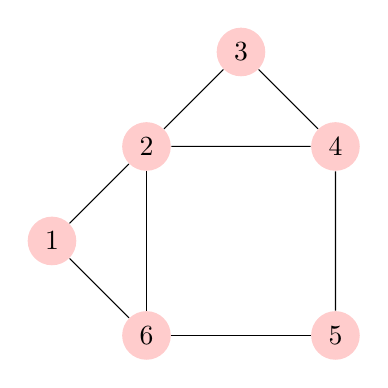
\begin{tikzpicture}
  [scale=.6,auto=left,every node/.style={circle,fill=red!20}]
  \node (n1) at (1,7) {1};
  \node (n2) at (3,9)  {2};
  \node (n3) at (5,11)  {3};
  \node (n4) at (7,9) {4};
  \node (n5) at (7,5)  {5};
  \node (n6) at (3,5)  {6};

  \foreach \from/\to in {n1/n2,n1/n6,n2/n3,n2/n4,n2/n6,n3/n4,n4/n5,n5/n6}
    \draw (\from) -- (\to);

\end{tikzpicture}
\caption{Can you list the cycles in this graph?}\label{day3g1}
\end{center}
\end{figure}

\textit{Before you turn the page, try to come up with an answer of your own!}

\newpage
\subsection*{Answer for the third day}
Ajur scratched his head and studied the graph that Rishnak showed him.  At length, he said, ``I think I see six cycles in the graph.'' He proceeded to list them.
\begin{itemize}
    \item Two cycles of length 3: $(1,2,6), (2,3,4)$
    \item One cycle of length 4: $(2,4,5,6)$
    \item Two cycles of length 5: $(2,3,4,5,6), (1,2,4,5,6)$
    \item One cycle of length 6: $(1,2,3,4,5,6)$
\end{itemize}

Rishnak was again pleased as this was the correct answer. He smiled and noticed that Ajur was getting restless, and so was Jura, so they called it a night.